
\section{Introduction} 

\renewcommand{\thefootnote}{\fnsymbol{footnote}}
\addtocounter{footnote}{-1}

Retrieval-augmented generation (RAG)~\cite{gao2023retrieval} has gained popularity as a way to enhance large language models (LLMs) with access to external knowledge, thereby reducing hallucination and improving accuracy in knowledge-intensive tasks. Recent research has extended this idea to knowledge graph retrieval-augmented generation (KG-RAG), where \emph{knowledge graphs (KGs)} are leveraged as the retrieval source. A KG is a structured representation of knowledge in the form of entities (nodes) and their relationships (edges) that encodes factual knowledge in a graph format.  Augmenting LLMs with KGs has proven effective not only in mitigating the knowledge bottleneck but also in improving reasoning performance over complex multi-hop relations and enhancing adaptation to continually evolving real-world information~\citep{Sun2024ToG, Luo2024RoG, Wang2025ReKnoS}. These properties make KG-RAG especially promising in high-stakes domains, such as medical consultation and legal analysis~\citep{zhao2025medrag, cui2024chatlawmultiagentcollaborativelegal}.

As shown in \Cref{fig1:overview}, a typical KG-RAG adopts a \emph{modular workflow} consisting of four subtasks: \emph{retrieval} to query facts from KGs, \emph{reasoning} to process retrieved information, \emph{reviewing} to verify logical consistency, and \emph{responding} to synthesize the answer~\citep{baek2023, Sun2024ToG, Luo2024RoG, Wang2025ReKnoS}. Each subtask is handled by specialized LLM modules through two main methods: (i) prompt-based modules with task-specific instructions, often including in-context demonstrations~\citep{baek2023}; and (ii) fine-tuned modules tailored to specific tasks (e.g., SPARQL generation~\citep{cotsparql2024,lee2025sparkle} or relation extraction~\citep{yao2019kgbert}) on specific KGs.

\begin{figure}[t!]
    % \vspace{-2em}
\centering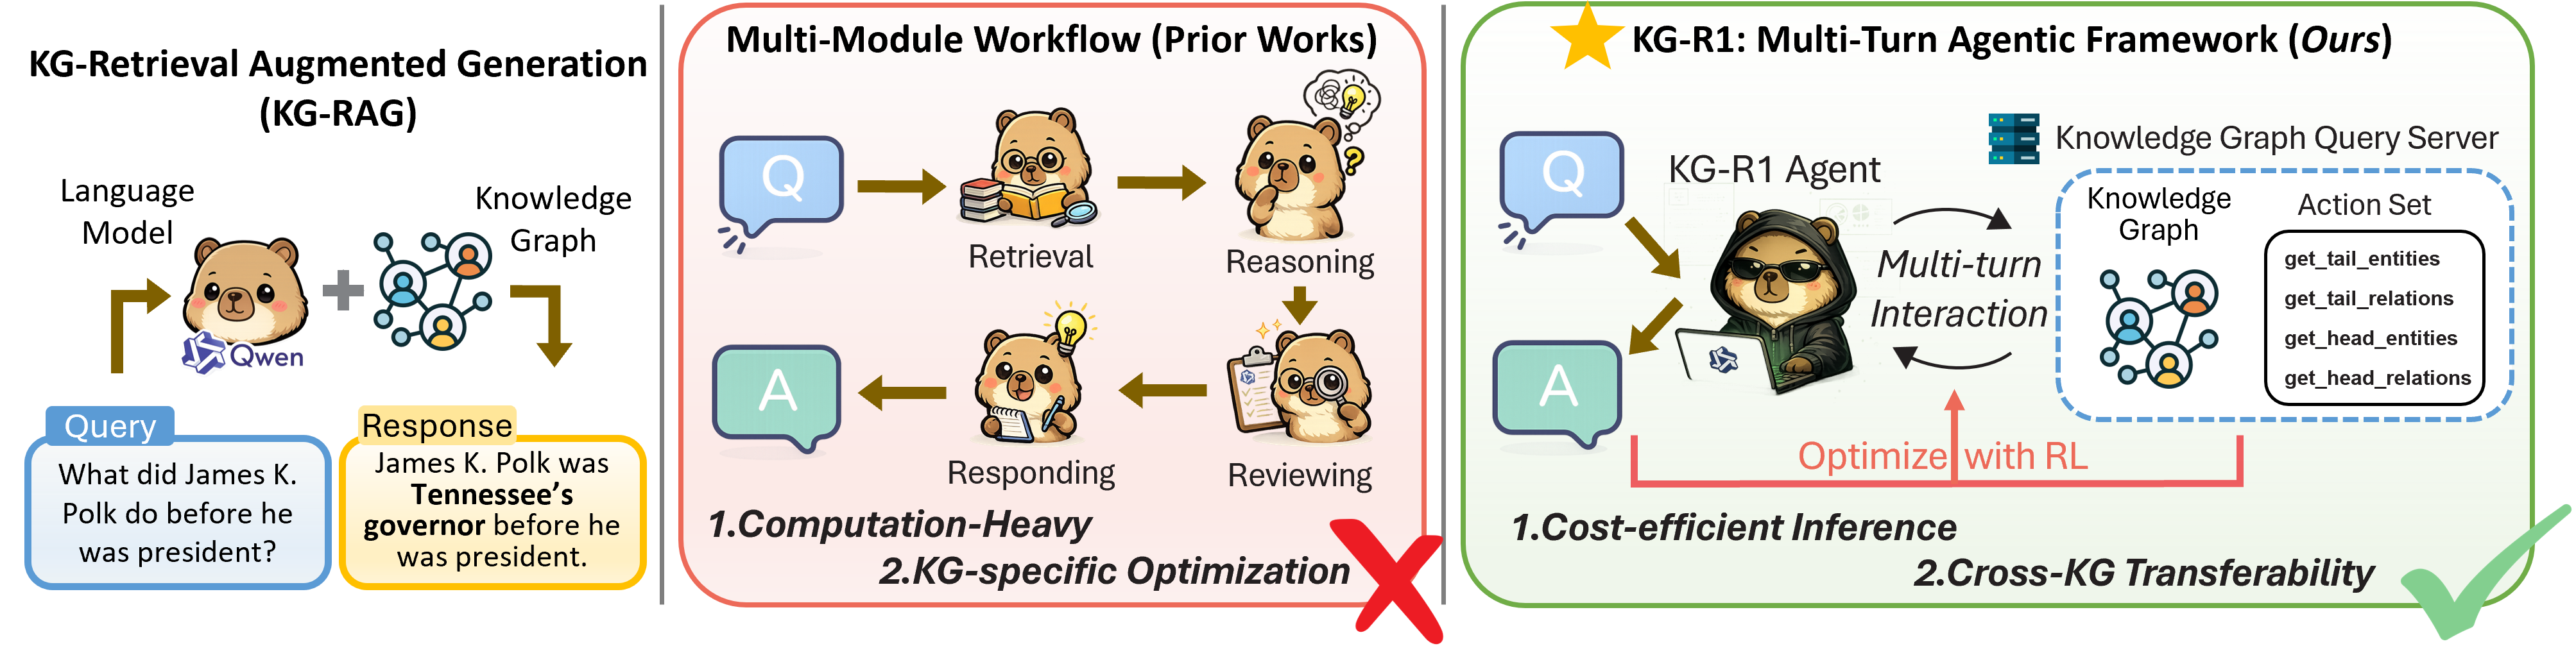
\includegraphics[width=1.0\textwidth]{Figures/overview.png}
    % \vspace{-1.5em}
    \caption{Overview of \framework{}, a multi-turn agentic KG-RAG framework. The framework enables cost-efficient inference and demonstrates strong cross-KG transferability.}
    \vspace{-1.5em}
    \label{fig1:overview}
\end{figure}

Despite improved reasoning accuracy, the real-world deployment of such workflows faces two key challenges: achieving high reasoning \textbf{effectiveness} while maintaining \textbf{efficiency}, and \textbf{generalization to new or updated KGs}. 
First, prompt-based methods that repeatedly call large foundation LLMs accumulate inference across stages and drive up latency, token usage, and compute (e.g., ToG \citep{Sun2024ToG} and ReKnoS \citep{Wang2025ReKnoS}; see left panel of \Cref{fig2}). Second, these prompted or fine-tuned modules are typically tuned to a particular KG’s domain and schema (entity types, relations, constraints), often via curated in-context examples or KG-specific fine-tuning. As a result, performance does not transfer reliably when the domain shifts, the schema changes, or the system is deployed on a new KG (e.g., RoG \citep{Luo2024RoG}; see right panel of \Cref{fig2}). 

\begin{wrapfigure}{r}{0.45\textwidth}
    \centering
    \vspace{-1.5em}
    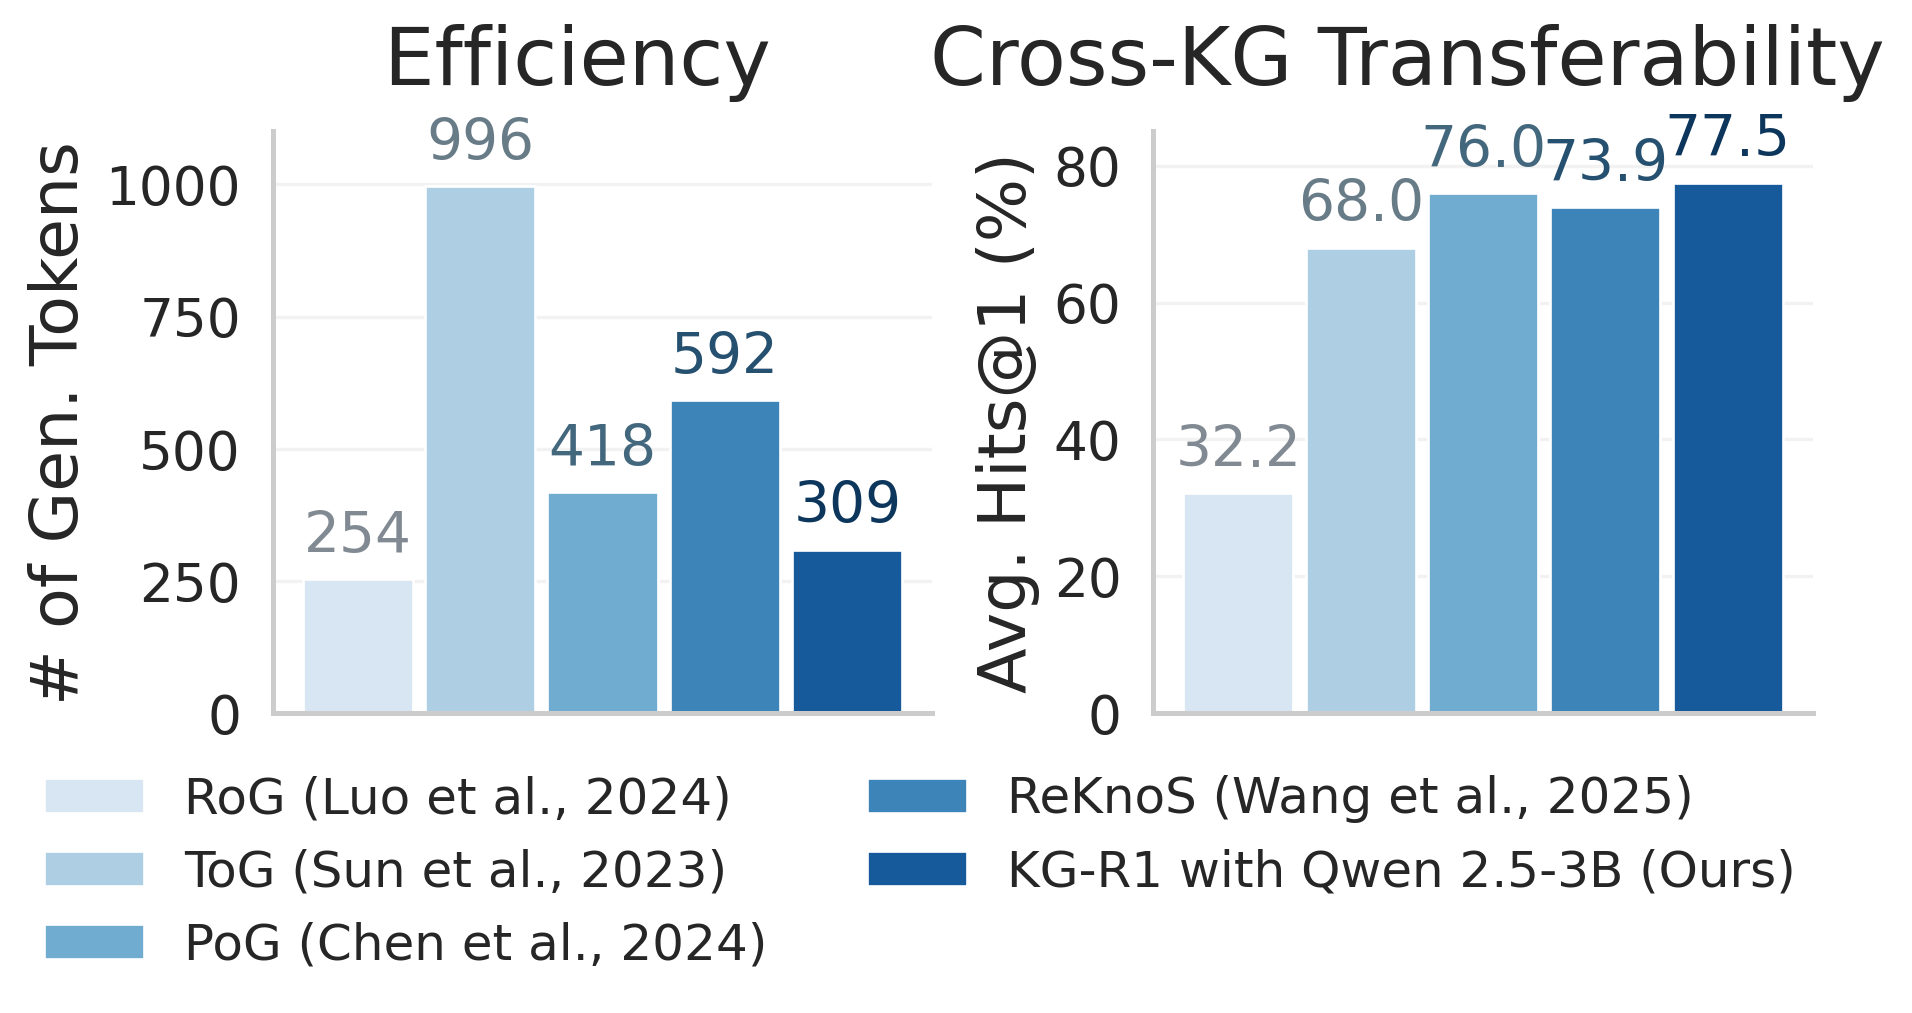
\includegraphics[width=\linewidth]{Figures/fig1_efficiency_and_transferability_v2.png}
    \vspace{-1.5em}
    \caption{Prior multi-module methods are costly and do not transfer well across KGs. \emph{Left:} mean end-to-end generated tokens per query on \dataset{WebQSP}~\citep{Yih2016WebQSP}. \emph{Right:} average Hits@1 over five out-of-training KGQA datasets (see \Cref{sec:exp2}). \framework{} achieves \emph{both} low token cost and strong cross-KG transferability.}
\label{fig2}
\vspace{-1.25em}
\end{wrapfigure}

To tackle these challenges, we introduce \textbf{\framework{}}, an agentic KG-RAG system that employs end-to-end multi-turn reinforcement learning~\citep{jin2025searchr1,zeng2025reinforcing, DeepSeek2025R1} to learn effective and transferable KG interaction policies. As shown in \Cref{fig1:overview}, the architecture of \framework{} has two components: a single LLM agent and a KG query server. The KG query server hosts the knowledge graph along with a set of retrieval actions. The LLM agent iteratively performs cycles of short reasoning followed by retrieval actions over multiple turns, with each decision informed by knowledge obtained from the KG retrieval server, and generates a final answer. 
By learning a unified interaction policy, \framework{} avoids redundant multi-module coordination and allocates computation adaptively across reasoning steps, leading to both improved effectiveness and reduced token usage.
\Cref{fig2} demonstrates that \framework{} achieves both high efficiency and strong cross-KG transferability \emph{simultaneously} using a 3B-parameter model, outperforming prior methods.
Our key contributions are summarized as follows:

\noindent \textbf{1. \framework{} Framework.} We introduce an agentic KG-RAG system (Section~\ref{sec:kg_r1}) that replaces multi-module pipelines with a \emph{single} agent for KG-RAG, running on a lightweight KG server. The agent alternates between reasoning and retrieval actions over multiple turns, with the end-to-end trajectory optimized by RL using both \emph{turn-wise} and \emph{outcome-based} reward signals. Turn-wise rewards evaluate individual action effectiveness and adherence to formatting, while global rewards measure answer quality and retrieval relevance.

\noindent \textbf{2. Effective and Efficient Inference.} By consolidating reasoning and retrieval into a \emph{single-agent, near-continuous} workflow, \framework{} achieves competitive reasoning accuracy with a small-parameter model while reducing token usage. This lowers latency and computational cost, making deployment feasible under tight budgets. Experiments demonstrate improved performance and efficiency compared to traditional multi-module workflows (Section~\ref{sec:exp1}). 

\noindent \textbf{3. Plug-and-play Transferability across Diverse KGs.} \framework{} can be easily transferred to diverse KGs and maintains strong KG-RAG performance (Section~\ref{sec:exp2}). The trained \framework{} agent generalizes to new KGs without retraining: backend KGs can be swapped without changing prompts, hyperparameters, or fine-tuning. This generalizability enables zero-shot transfer to unseen KGs.



 






